\providecommand{\setflag}{\newif \ifwhole \wholefalse}
\setflag
\ifwhole\else

% Typography and geometry ----------------------------------------------------
\documentclass[letterpaper]{scrbook}
\usepackage[inner=3cm,top=2.5cm,outer=3.5cm]{geometry}

\renewcommand\familydefault{bch}
\usepackage[utf8]{inputenc}
\usepackage{microtype}
\usepackage[small]{caption}
\usepackage[small]{titlesec}
\raggedbottom

% Graphics -------------------------------------------------------------------
\usepackage[pdftex]{graphicx}
\graphicspath{{_include/}}
\DeclareGraphicsExtensions{.png,.pdf}

% Code formatting ------------------------------------------------------------
\usepackage{fancyvrb}
\usepackage{courier}
\usepackage{listings}
\usepackage{color}
\usepackage{alltt}


\definecolor{comment}{rgb}{0.60, 0.60, 0.53}
\definecolor{background}{rgb}{0.97, 0.97, 1.00}
\definecolor{string}{rgb}{0.863, 0.066, 0.266}
\definecolor{number}{rgb}{0.0, 0.6, 0.6}
\definecolor{variable}{rgb}{0.00, 0.52, 0.70}
\lstset{
  basicstyle=\ttfamily,
  keywordstyle=\bfseries, 
  identifierstyle=,  
  commentstyle=\color{comment} \emph,
  stringstyle=\color{string},
  showstringspaces=false,
  columns = fullflexible,
  backgroundcolor=\color{background},
  mathescape = true,
  escapeinside=&&,
  fancyvrb
}
\newcommand{\code}[1]{\lstinline!#1!}
\newcommand{\f}[1]{\lstinline!#1()!}



% Links ----------------------------------------------------------------------

\usepackage{hyperref}
\definecolor{slateblue}{rgb}{0.07,0.07,0.488}
\hypersetup{colorlinks=true,linkcolor=slateblue,anchorcolor=slateblue,citecolor=slateblue,filecolor=slateblue,urlcolor=slateblue,bookmarksnumbered=true,pdfview=FitB}
\usepackage{url}

% Tables ---------------------------------------------------------------------
\usepackage{longtable}
\usepackage{booktabs}

% Miscellaneous --------------------------------------------------------------
\usepackage{pdfsync}
\usepackage{appendix}

\usepackage[round,sort&compress,sectionbib]{natbib}
\bibliographystyle{plainnat}


\title{ggplot2}
\author{Hadley Wickham}

\begin{document}
\fi


\chapter{Polishing your plot}

\section{Introduction}

In ggplot, the appearance and the structure of the plot are quite separate.  This is different to base and lattice graphics in that you do not specify the appearance of the plot while you are creating it (defining its structure).  In base and lattice graphics, most functions take a very large number arguments that specify the finer points of appearance, which can make the functions complicated and hard to understand.  Instead, in ggplot you create the plot in one step, and then {\em after} it has been created you can edit every detail of the rendering.  

The are two ways to do this: common options are exposed by the {\tt ggopt} function, or you can use the grid package to modify the graphical output of ggplot.  The few options provided by {\tt ggopt} allow you to easily modify the most commonly tweaked parts of ggplot graphics, but for more control you can use the power of grid to delve into the dark depths of {\tt ggplot} and tweak to your heart's content.

What is grid?  It's the graphics engine that powers ggplot.  It is responsible for drawing the graphic object onto the screen or other output device.  It provides a system of viewports, which define regions on the plot and the coordinate systems inside.  A useful reference is \url{http://www.stat.auckland.ac.nz/~paul/RGraphics/chapter5.pdf} a sample chapter from Paul Murrell's Grid Graphics.

Please remember that ggplot has been carefully designed to provide perceptually well-founded defaults, and you should think carefully about what you are doing before you make any big changes.  Some particularly good references to consult are:

\begin{itemize}
	\item \citet{cleveland:1993,cleveland:1987,cleveland:1994} for research on how plots are perceived and the best ways to encode data.
	\item \citet{tufte:2006,tufte:1990,tufte:1997,tufte:2001} for how to make beautiful, data-rich, graphics.
  % \item \citet{bertin:1983,bertin:1967}, especially for maps.
	\item \citet{brewer:1994,brewer:1994a} for how to colours that work well in a wide variety of situations, particularly for area plots.
	\item \citet{carr:1999,carr:1994,carr:2002}, for the use of colour in general.
\end{itemize}

This chapter can not hope to provide a comprehensive introduction to grid, but should hopefully provide enough examples to get you going.   I highly recommend the book ``R Graphics'' \citep{murrell:2005}, by the author of grid,  as a companion to this chapter.   

The grobs (graphical objects) used in this chapter are a bit different to the geoms (geometric objects) used in previous chapters.  A grob is the object that is actually drawn onto the screen, while a geom is a more abstract object which describes the type of object used to draw a plot.  An example may make this more clear. In a line plot, the geom describes that the data should be visualised with a line, and the grobs draw the line itself, as well as the other lines that appear in the grid and axes.



\section{Options}\label{sec:options}

ggplot provides convenient access to a select set of commonly used options, described in Table \ref{tbl:options}.  These options are described in more depth, with many examples, in the online documentation {\tt ?ggopt}.
There are two ways to set options:

\begin{itemize}
  \item Globally (for all plots), using {\tt ggopt}.  For example {\tt ggopt(grid.fill = "white")}.   Global options are applied when a plot is rendered, not when it is created.  This lets you experiment with plot structure and appearance independently.

  \item Locally (for one plot), using \$ or {\tt update}.  For example, {\tt p\$grid.fill <- "white"}, or {\tt update(p, grid.fill = "white")}.  The first modifies the object in place, while the second creates a modified copy. Local options override the more general global options.
\end{itemize}     


\begin{table}
\begin{tabular}{lll}
Option & Valid values & Details \\
\hline
background.fill    & any colour & Background fill colour behind entire plot\\
background.colour  & any colour & \\
grid.colour        & any colour & Colour of grid lines within panel \\
grid.fill          & any colour & Panel background colour \\
strip.gp           & gpar object & Graphical parameters used for strip. Colour and fill of most interest \\
strip.text.gp      & any colour & Graphical parameters used for strip text. \\
strip.text         & a function & Function should accept two arguments, variable and value and return a character vector of length one. Function which determines how strip labels are formatted \\
legend.position    & left, right, top, bottom, none, c(x, y) & Position of legend.  Can use numeric vector of length 2 to set position of centre of length, units are npc relative to whole plot viewport. \\
aspect.ratio       & a number or NULL & Aspect ratio of plot. \\
\hline
\end{tabular}
  \caption{ggplot options}
  \label{tbl:options}
\end{table}

\begin{table}
  \begin{center}
  \begin{tabular}{ll}
  Option & Description \\
  \hline
  fill, col & Background and foreground colours.  You can supply a named colour (see {\tt ?colors}) or a hex string of the form \#RRGGBBAA or \#RRGGBB. \\
  lty & Line type: solid, dotted, dashed etc. \\
  lwd & Width of line, in points. \\
  fontfamily, fontface & Refer to R-news article \\
  fontsize & Font size, in points.  
    
  \end{tabular}
  \end{center}
  \caption{gpar specifications.  See {\tt ?gpar} for more details}
  \label{tbl:gpar}
\end{table}

The following example demonstrates some of the possibilities.

% decumar<<< 
% dsmall <- diamonds[sample(1:nrow(diamonds), 1000), ]
% doptions(height=3, width=4)
% interweave({
% # Always a good idea to save existing options before making
% # radical changes
% old <- ggopt(grid.colour="grey50", grid.fill="white")
% qplot(carat, price, data=dsmall)
% (p <- qplot(cut, clarity, data=dsmall, geom="jitter"))
% # Only changes the current plot
% p$grid.colour <- "darkgreen"
% p
% # Restore old settings:
% ggtheme(old)
% p
% })
% |||
\begin{alltt}
> old <- ggopt(grid.colour = "grey50", grid.fill = "white")
> qplot(carat, price, data = dsmall)
\includegraphics[scale=1]{7f8d370a14179d509879f35839b54ea9}

> (p <- qplot(cut, clarity, data = dsmall, geom = "jitter"))
\includegraphics[scale=1]{5830a37fc4252db571b25f373c8f141f}

> p$grid.colour <- "darkgreen"
> p
\includegraphics[scale=1]{656e171fb34b88b28f6789aa9ad535e6}

> ggtheme(old)
> p
\includegraphics[scale=1]{656e171fb34b88b28f6789aa9ad535e6}

\end{alltt}
% >>>

\subsection{Themes}\label{sub:themes}

Like lattice, it is also possible to create a theme which encapsulates multiple options.  A theme is a very simple structure, just a list of multiple options, so it's  easy to create your own.  One theme is included by default: {\tt theme\_bw}, which sets up a white background with black grid lines.  You can use a theme with {\tt ggtheme(theme)}, or for a single plot {\tt update(plot, theme)}.

% decumar<<< 
% interweave({
% ggtheme(theme_bw)
% qplot(carat, price, data=dsmall)
% })
% |||
\begin{alltt}
> ggtheme(theme_bw)
> qplot(carat, price, data = dsmall)
\includegraphics[scale=1]{7f8d370a14179d509879f35839b54ea9}

\end{alltt}
% >>>

\section{Modifying the plot with grid}

There are three principle ways to modify a plot:

\begin{itemize}
  \item Edit existing objects on the plot
  \item Add annotations to the plot
  \item Arrange multiple plots on a single page
\end{itemize}

To annotate or edit a plot, you first need to figure out what you want to change, and what it is called.  If you are annotating plots, you will need to know the name of the appropriate viewport.  If you are editing plots, you will need to know the name of the appropriate grob.  This following sections describe the structure of the plot and how to modify it

\subsection{Editing existing objects on the plot}

\subsection{Grob names}

To edit existing grobs, you need to know their names.  Grob names have three components: the name of the grob, the class of the grob, and a unique numeric suffix.  The three components are joined together with ``.'' to give a name like {\tt title.text.435} or {\tt ticks.segments.15}.  These three components ensure that all grob names are unique, and allow you to select multiple grobs with the same name at the same time.

% TODO: Update me! with grid.ls

You can see a list of all the grobs in the current plot with {\tt grid.ls()}.  If you only want to see the ggplot name of the grob, {\tt grid.ls(only.name=TRUE)} will reduce a lot of the output.  Here's an example after drawing the previous plot:

\begin{alltt}
plot-surrounds::
 background
 plot::
  background
  guide:: (background, major-horizontal, major-vertical, 
           minor-horizontal, minor-vertical, border)
  xaxis::
   ticks
   labels:: (label, label, label, label, label, label, label, label)
  yaxis::
   ticks
   labels:: (label, label, label, label, label)
  geom_point
 ylabel
 xlabel
 title
\end{alltt}

Notice that the grobs are arranged in a hierarchical manner. 

The most important components are:

\begin{itemize}
  \item {\tt guide}, the internal guides within a panel (background, and grid lines)

  \item {\tt xaxis} and {\tt yaxis}, the axes, containing {\tt labels} and {\tt ticks}.

	\item Axis labels and title: {\tt xlabel}, {\tt ylabel}, {\tt title}.

  \item The geom displayed in the plot: {\tt geom\_point}.

	\item Another important component not shown in this example are {\tt strip}s: containing the {\tt background} background fill and {\tt label}.

\end{itemize}

\subsection{Modifying grobs}

Most of the difficulty in modifying stuff on the plot is figuring out the name of the grob you want to modify, and once you have that you can use {\tt grid.gedit}.  {\tt grid.gedit} does two things: it finds the grobs you want to modify, and then changes their appearance.  

You describe which grobs to modify with a gPath.  A gPath can either be a string specifying a single grob name, or a sequence of grob names with the {\tt gPath} function.  Using a string will find all grobs with that name regardless of their position in the hierarchy.  For example, {\tt "label"} will find all grobs called label, regardless of where they are.  To be more specific, using {\tt gPath("parent", "child")} will only find grobs named ``child'' with a parent called ``parent''.  For example, {\tt gPath("xaxis", "label")} will locate only labels on the x-axis.

Modifying a grob requires some knowledge of the different parameters of the grob.  This is where the second part of the grob name is useful, as it will tell you whether you are modifying a line, or a rect or a text grob.  You can get more information by looking at the documentation for that grob, eg. {\tt ?grid.rect, ?grid.text, ?grid.lines}   All grobs share a common set of graphical parameters described in Table \ref{tbl:gpar}.  Note that grid graphic parameters (gpar) have difference argument names than the usual ggplot names (cex instead of size, pch instead of shape, col instead of colour)

In this example, we edit the font of all labels.

\begin{alltt}
qplot(mpg, wt, data=mtcars, facets = . ~ cyl)
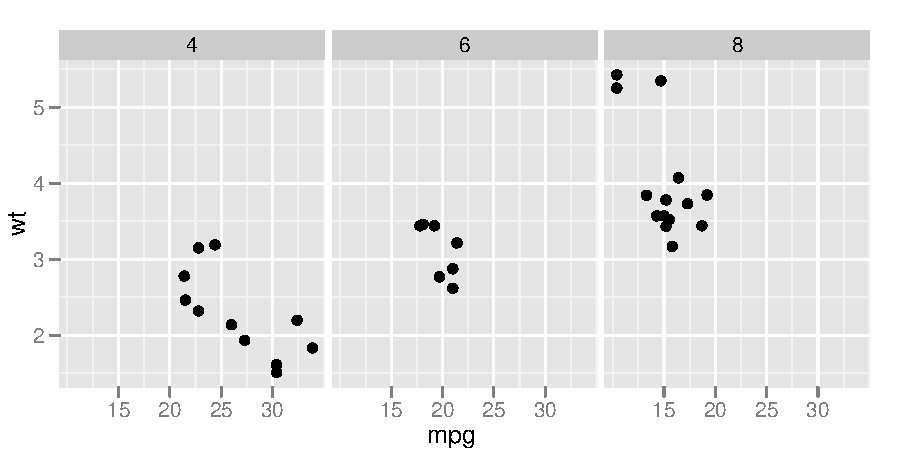
\includegraphics[scale=0.5]{grid1}
grid.gedit("label", gp=gpar(fontsize=14, col="red"))
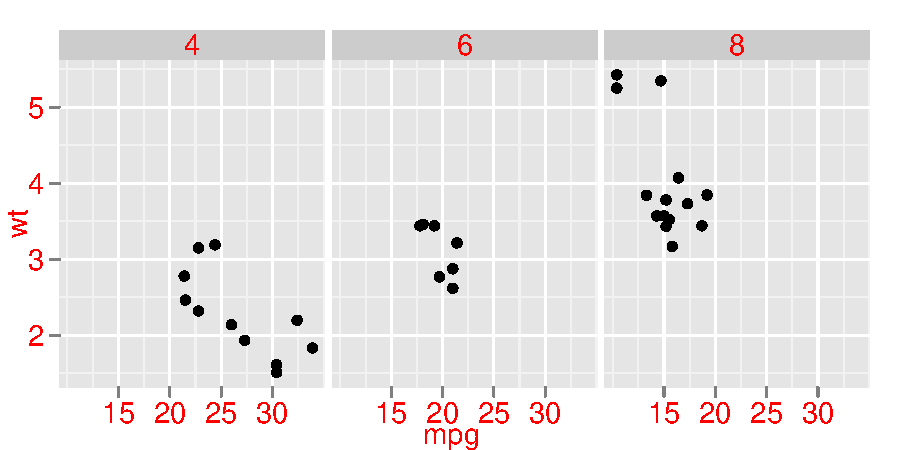
\includegraphics[scale=0.5]{grid2}
\end{alltt}
% dev.save("_include/grid1.pdf")
% dev.save("_include/grid2.pdf")

To edit just one type of label, we need to use the hierarchy of grobs and the {\tt gPath} function:

\begin{alltt}
qplot(mpg, wt, data=mtcars, facets = . ~ cyl)
grid.gedit(gPath("strip","label"), gp=gpar(fontface="bold"))
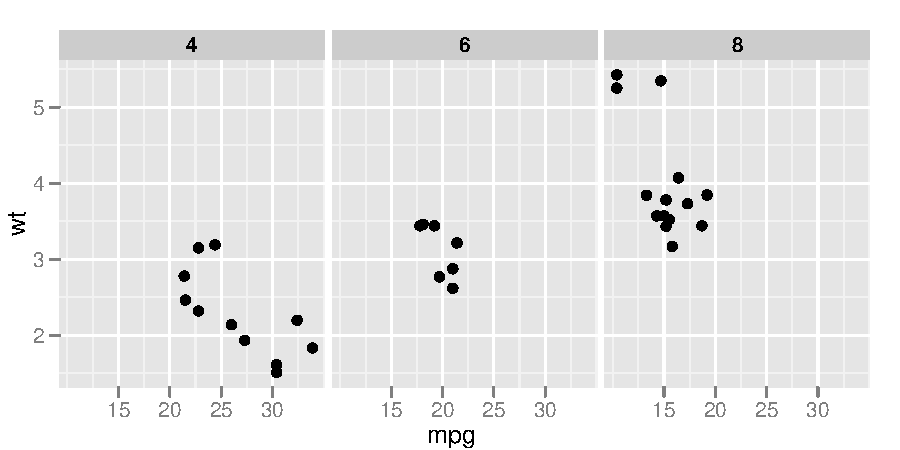
\includegraphics[scale=0.5]{grid3}
grid.gedit(gPath("yaxis", "labels"), gp=gpar(col="red"))
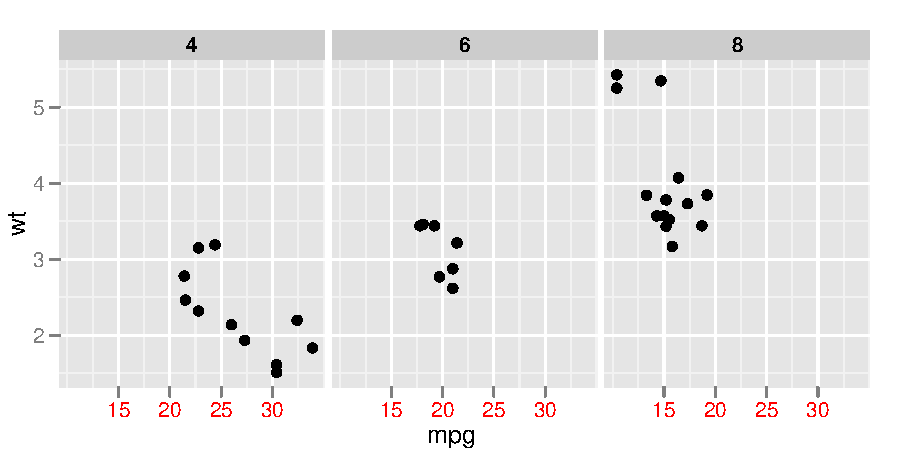
\includegraphics[scale=0.5]{grid4}
\end{alltt}

% \subsection{Removing grobs}\label{ssub:removing_grobs}
% 
% You can use {\tt grid.remove} to completely remove a grob.
% 
% \begin{alltt}
% qplot(mpg, wt, data=mtcars, facets = . ~ cyl)
% 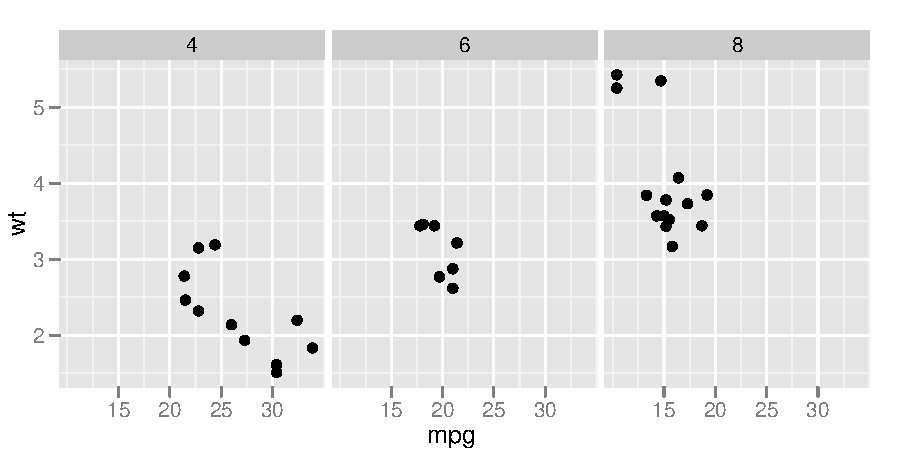
\includegraphics[scale=1]{grid1}
% grid.gremove(gPath("strip", "background"))
% \includegraphics[scale=1]{grid5}
% grid.gremove(gPath("guide", "background"))
% \includegraphics[scale=1]{grid6}
% grid.gremove("major")
% \includegraphics[scale=1]{grid7}
% grid.gremove("axis")
% \end{alltt}

% FIXME: check labelled and modified axes are the same

\subsection{Adding annotations}\label{sec:adding_annotation}

Many annotations can be done with {\tt geom\_text}, {\tt geom\_abline}, {\tt geom\_vline} and {\tt geom\_hline}, so try those first.  If you need more flexibility you can add annotations with grid.  When you add annotations to a plot you need to specify where they will appear.  In grid this is described by a system of viewports.  Different viewports describe different regions of output on the plot, for example, the axes, the plotting region and the faceting strips.

The structure of viewports will vary slightly from plot to plot, depending on the type of faceting.  For a plot produced with {\tt facet\_grid}, the default, the viewports are described below.  For other types of faceting, the details will vary slightly, and are described in the documentation for that faceting system.  

The {\tt layout} viewport contains the meat of the plot: strip labels, axes and faceting panels.  The viewports are named according to their role and their position.  A viewport name is made up of a prefix (listed below) which describes the contents of the viewport, and x and y position (counting from bottom left) separated by ``\_''.

\begin{itemize}
  \item {\tt strip\_h}: horizontal strip labels
  \item {\tt strip\_v}: vertical strip labels
  \item {\tt axis\_h}: horizontal axes
  \item {\tt axis\_v}: vertical axes
  \item {\tt panel}: faceting panels
\end{itemize}

% Figure \ref{fig:viewports} shows this diagrammatically.
% 
% \begin{figure}[htbp]
%   \centering
%     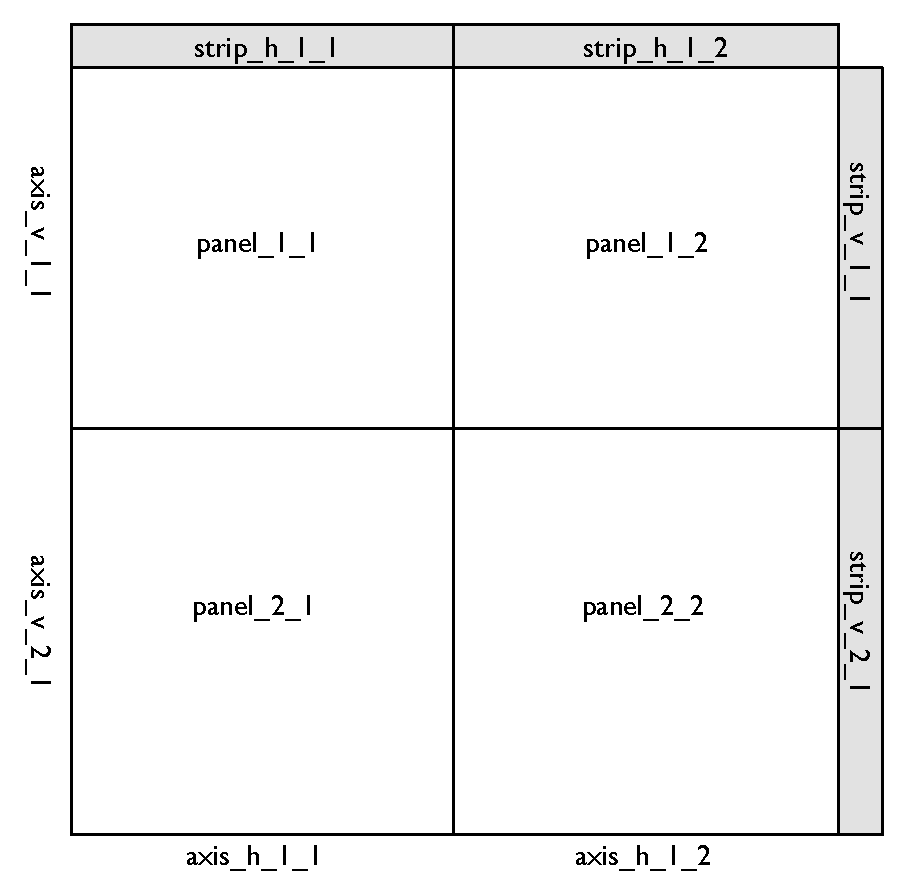
\includegraphics[scale=0.65]{7-grid-viewports.pdf}
%   \caption{Diagram showing the structure and names of viewports.}
%   \label{fig:viewports}
% \end{figure}

You can see all the viewports on the current plot by typing {\tt current.vpTree(all=TRUE)}.

\begin{sidebar}
Unfortunately there is a bug in grid which currently prevents all the viewports being accessed and displayed.  You can get around this by printing only the bare necessities of the plot:

\begin{alltt}
p <- qplot(wt, mpg, data=mtcars, colour=cyl)
print(p, pretty = FALSE)
current.vpTree(all=TRUE)
\end{alltt}  

\end{sidebar}

To add annotations to a plot you have to specify the viewport when you add extra grobs.  For example:

\begin{alltt}
p <- qplot(wt, mpg, data=mtcars, colour=cyl)
print(p, pretty=FALSE)
grid.circle(vp="layout::panel_1_1")
\end{alltt}

Panel viewports will have a coordinate system set up for points, while x- and y- axes will only have one dimension defined.  For example, on the x-axis there will be native coordinates for the x-dimension, but not the y-dimension.

\begin{alltt}
p <- qplot(wt, mpg, data=mtcars, colour=cyl)
print(p, pretty=FALSE)
grid.lines(x=unit(c(0,1), "npc"), y=unit(23, "native"), vp="layout::panel_1_1")
grid.lines(x=unit(c(0,1), "npc"), y=unit(23, "native"), vp="layout::axis_v_1_1")
\end{alltt}


% Non-Cartesian coordinate systems

\subsection{Customising layout}\label{sec:grid_layout}

By default, showing a {\tt ggplot} object at the R command prompt will display to the screen.  To exercise more control, you can call {\tt print} explicitly.  This section describes some of the things you can do.  For more details see {\tt ?print.ggplot} and {\tt ?ggplot\_print}.

If you just want the plot (no labels, titles or legends) you can use {\tt pretty = FALSE}

\begin{alltt}
p <- qplot(wt, mpg, data=mtcars, colour=cyl)
print(p, pretty = FALSE)
\end{alltt}

By default, {\tt ggplot} always clears the screen and draws to the entire device.  You customise this in two ways. One way is to setup a viewport and push it on to the display, then draw the plot with {\tt newpage=FALSE}. {\tt pushViewport} adds the viewport to the list of viewports on the display.   Afterwards, {\tt upViewport} returns you to the viewport for the entire page, preparing you for the next set of output.

\begin{alltt}
p <- qplot(wt, mpg, data=mtcars, colour=cyl)
grid.newpage()
pushViewport(viewport(height=0.4, width=0.4, x=0.4, y=0.8))
print(p, newpage=FALSE, pretty=FALSE)
upViewport()
\end{alltt}

Alternatively, you can set up your own set of viewports, and then specify which one the plot should be drawn to.  Here we use {\tt upViewport} before displaying the plot so we are in the top level viewport before we start plotting.

\begin{alltt}
grid.newpage()
pushViewport(viewport(height=0.5, width=0.5, x=0.5, y=0.5, name="small", angle=40))
upViewport()
print(p, vp="small")
\end{alltt}

Obviously, this is very useful if you want to layout plots in a complicated grid.  In this case, {\tt grid.layout} is very useful, as it allows you to set up a grid of viewports with arbitrary heights and widths.  You still need to create each viewport, but instead of explicitly specifying the position and size, you can specify the row and column of the layout.

\begin{alltt}
p <- qplot(wt, mpg, data=mtcars, colour=cyl)

vplayout <- function(x, y) viewport(layout.pos.row=x, layout.pos.col=y)
grid.newpage()
pushViewport(viewport(layout=grid.layout(3,3)))

print(p, vp=vplayout(1,1))
print(p, vp=vplayout(2:3,2:3))
print(p, vp=vplayout(1, 2:3))
print(p, vp=vplayout(2:3, 1))
\end{alltt}

This is useful for arranging plots in a wider range of ways than what you can do with faceting.   You should be careful to ensure that scales are consistent over the different plots.  There is currently no easy way to do this, except to keep track of the maximum and minimum yourself, and then manually set the scales of the plot.

% How to access legends indepentently of the plot, with example showing multiple plots with common scales and legend added manually


\ifwhole
\else
  \nobibliography{/Users/hadley/documents/phd/references}
  \end{document}
\fi
